
\section{HAT Implications}
\label{sec:evaluation}

With an understanding of which guarantees are HAT-compliant, in this
section, we analyze the implications of these results for existing
systems and briefly study HAT systems on public cloud
infrastructure. Specifically:

\begin{myenumerate}\vspace{-.5em}
\item We revisit traditional database concurrency control with a focus
  on coordination costs and on high availability.
\item We examine the properties required by an OLTP application based
  on the TPC-C benchmark.
\item We perform a brief experimental evaluation of HAT versus non-HAT
  properties on public cloud infrastructure.
\end{myenumerate}

\subsection{Existing Algorithms}
\label{sec:eval-existing}

Most existing database transaction and concurrency control algorithms
are not designed for high availability and often presume a
single-server deployment or a requirement for serializability. In this
section, we briefly discuss design decisions and algorithmic details
that preclude high availability.

\vspace{.5em}\noindent\textbf{Serializability} To establish a serial
order on transactions, algorithms for achieving serializability of
general-purpose read-write transactions in a distributed
setting~\cite{bernstein-book, davidson-survey, wisemann-survey}
require at least one RTT before committing. As an
example, traditional two-phase locking for a transaction of length $T$
may require $T$ \texttt{lock} operations and will require at least one
\texttt{lock} and one \texttt{unlock} operation.  In a distributed
environment, each of these lock operations requires coordination,
either with other database servers or with a lock service. If this
coordination mechanism is unavailable, transactions cannot safely
commit. Similarly, optimistic concurrency control requires
coordinating via a validation step, while deterministic transaction
scheduling~\cite{deterministic-scheduling} requires a
scheduler. Serializability under multi-version concurrency control
requires checking for update conflicts. All told, the reliance on a
globally agreed total order necessitates a minimum of one round-trip
to a designated master or coordination service for each of these
classic algorithms.  The cost of round trips will be determined by the
deployment environment, as we saw in Section~\ref{sec:motivation}; we
will demonstrate this cost on public cloud infrastructure in
Section~\ref{sec:prototype}.

\vspace{.5em}\noindent\textbf{Non-serializability} Most existing
distributed implementations of weak isolation are not highly
available. Lock-based proposals such as those used to provide weak
isolation in Gray's original proposal~\cite{gray-isolation} do not
degrade gracefully in the presence of partial failures. (Note,
however, that lock-based protocols \textit{do} offer the benefit of
recency guarantees.) While multi-versioned storage systems allow for a
variety of transactional guarantees, few offer traditional weak
isolation (e.g., non-``tentative update'' schemes) in this context.
The MDCC~\cite{mdcc} protocol offers Read Committed isolation with
Lost Update avoidance but is similarly unavailable due to its reliance
on preventing write conflicts. Chan and Gray's read-only transactions
have item-cut isolation with causal consistency and TA (session
\textit{PL-2L}~\cite{adya}) but are unavailable in the presence of coordinator
failure and assume serializable update transactions~\cite{readonly};
this is similar to read-only and write-only transactions more recently
proposed by Eiger~\cite{eiger}. Causal Serializability offers a
similar model (with unavailable implementation): causal consistency
with a variant of Read Uncommitted between transactions that write to
the same data item~\cite{raynal-causal}.  Brantner's S3
database~\cite{kraska-s3} and Bayou~\cite{sessionguarantees} can all
provide variants of session \textit{PL-2L} with high availability, but none
provide this HAT functionality without substantial
modification. Swift~\cite{swift} and bolt-on causal
consistency~\cite{bolton} are closest to providing maximum sticky HAT
semantics. As we have seen, it is possible to implement many
guarantees weaker than serializability---including guarantees that are
achievable with high availability---and still not achieve high
availability.

\subsection{Application Requirements}

Thus far, we have largely ignored the question of when HAT semantics
are useful (or otherwise are too weak). As we showed in
Section~\ref{sec:hats}, the main cost of high availability and low
latency comes in the inability to prevent Lost Update, Write Skew, and
provide recency bounds. In this section, we attempt to understand when
these guarantees matter both abstractly and in a representative
transactional application based on the TPC-C benchmark~\cite{tpcc}.

\vspace{.5em}\noindent\textbf{Commutativity and Monotonicity} As
evidenced by the CALM Theorem~\cite{calm} and by Commutative and
Replicated Data Types~\cite{crdt}, if updates logically commute, then
they can often be safely performed in different orders at different
replicas. Accordingly, as long as all writes are delivered to all
replicas, then a system executing monotonic logic may not suffer from
application-level consistency anomalies as a result of Lost Update or
Write Skew anomalies. However, applications with non-monotonic state
mutation will not, in general, be able to maintain application-level
consistency constraints with HATs alone---in particular, applications
requiring bounded update visibility latency should opt for
unavailability.

\vspace{.5em}\noindent\textbf{TPC-C} To better understand the impact
of HAT-compliance in an application context, we consider a concrete
application: the TPC-C benchmark. In brief, we find that four of five
transactions can be executed with HATs, while the fifth may require
unavailability.

TPC-C consists of five transactions, capturing the operation of a
wholesale warehouse, including sales, payments, and deliveries. Two
transactions---\textit{Order-Status} and \textit{Stock-Level}---are
read-only and can be executed safely with HATs. Clients may read stale
data, but this does not violate TPC-C requirements and clients will
read their writes if they are sticky-available. Another transaction
type, \textit{Payment}, updates running balances for warehouses,
districts, and customer records and provides an audit trail. The
transaction is monotonic---increment- and append-only---so all balance
increase operations commute, and TA allows the maintenance of
foreign-key integrity constraints (e.g., via \texttt{UPDATE/DELETE
  CASCADE}).

\vspace{.5em}\noindent\textit{New-Order and Delivery.} While three out of
five transactions are easily achievable with HATs, the remaining two
transactions are not as simple. The New-Order transaction places an
order for a variable quantity of data items, updating warehouse stock
as needed. It selects a sales district, assigns the order an ID
number, adjusts the remaining warehouse stock, and writes a
placeholder entry for the pending order. The Delivery transaction
represents the fulfillment of a New-Order: it deletes the order from
the pending list, updates the customer's balance, updates the order's
carrier ID and delivery time, and updates the customer balance.

\vspace{.5em}\noindent\textit{IDs and decrements.} The New-Order transaction presents two challenges: ID assignment and
stock maintenance. First, each New-Order transaction requires a unique
ID number for the order. We can create a unique number by, say,
concatenating the client ID and a timestamp. However, the TPC-C
specification requires order numbers to be \textit{sequentially}
assigned within a district, which requires preventing Lost
Update. Accordingly, HATs cannot provide compliant TPC-C execution but
can still maintain uniqueness constraints. Second, the New-Order
transaction decrements inventory counts: what if the count becomes
negative?  Fortunately, TPC-C New-Order restocks each item's inventory
count (increments by 91) if it would become negative as the result of
placing an order. This means that, even in the presence of concurrent
New-Orders, an item's stock will never fall below zero. This is TPC-C
compliant, but a HAT system might end up with more stock than in a
non-HAT-compliant implementation.

\vspace{.5em}\noindent\textit{TPC-C Non-monotonicity.} The Delivery
transaction is challenging due to non-monotonicity. Each Delivery
deletes a pending order from the New-Order table and should be
idempotent in order to avoid billing a customer twice; this implies a
need to prevent Lost Update. This issue can be avoided by moving the
non-monotonicity to the real world---the carrier that picks up the
package for an order can ensure that no other carrier will do so---but
cannot provide a correct execution with HATs alone. However, according
to distributed transaction architects~\cite{entitygroup}, these
compensatory actions are relatively common in real-world business
processes.

\vspace{.5em}\noindent\textit{Integrity Constraints.} Throughout execution, TPC-C also requires the maintenance of several
integrity constraints. For example, Consistency Condition 1 (3.3.2.1)
requires that each warehouse's sales count must reflect the sum of its
subordinate sales districts. This integrity constraint spans two
tables but, given the ability to update rows in both tables atomically
via TA, can be easily maintained. Consistency Conditions 4 through 12
(3.3.2.4-12) can similarly be satisfied by applying updates atomically
across tables. Consistency Conditions 2 and 3 (3.3.2.2-3) concern
order ID assignment and are problematic. Finally, while TPC-C is not
subject to multi-key anomalies, we note that many TPC-E isolation
tests (i.e., simultaneously modifying a product description and its
thumbnail) are also achievable using HATs.

\vspace{.5em}\noindent\textit{Summary.} Many---but not all---TPC-C
transactions are well-served by HATs. The two problematic
transactions, New-Order and Payment, rely on non-monotonic state
update. The former can be modified to ensure ID uniqueness but not
sequential ID ordering, while the latter is inherently non-monotonic,
requiring external compensation or stronger consistency
protocols. Based on these experiences and discussions with
practitioners, we believe that HAT guarantees can provide useful
semantics for a large class of application functionality, while a
(possibly small) subset of operations will require stronger,
unavailable properties.

\subsection{Experimental Costs}
\label{sec:prototype}

To further understand the performance implications of HAT guarantees
in a real-world environment, we implemented a HAT database
prototype. Across a range of deployments on public cloud
infrastructures, we found that, as Section~\ref{sec:latency}'s
measurements suggested, ``strongly consistent'' algorithms incur
substantial latency penalties: over WAN, 10 to 100 times higher than
their HAT counterparts. Given recent algorithms for providing
causal consistency~\cite{bolton, cops, swift}, we focus our HAT
analysis on TA (algorithm from Section~\ref{sec:ta}, described in
greater detail
in Appendix B
%in our Technical Report~\cite{hat-tr}
), which we believe to be the
most interesting of our algorithms. We find that HAT
properties---while more resource-intensive than basic eventual
consistency---scale well to many servers.

\vspace{.5em}\noindent\textit{Implementation.} Our prototype database
is a partially replicated (hash-based, partitioned) key-value backed
by LevelDB and implemented in Java using Apache Thrift. It currently
supports eventual consistency (hereafter, \texttt{eventual};
last-writer-wins RU with standard all-to-all anti-entropy between
replicas) and HAT RC and TA with RC guarantees (hereafter,
\texttt{TA}). It also supports non-HAT operation whereby all
operations for a given key are routed to a (randomly) designated
\texttt{master} replica for each key (guaranteeing single-key
linearizability, as in Gilbert and Lynch's CAP Theorem
proof~\cite{gilbert-cap} and in PNUTS~\cite{pnuts}'s
\texttt{read-latest} operation; hereafter, \texttt{master}) as well as
distributed two-phase locking. Servers are durable: they synchronously
write to LevelDB before responding to client requests, while new
writes in TA are sent to a write-ahead log, which is synchronously
flushed to disk.

\vspace{.5em}\noindent\textit{Configuration.} We deploy the database
in \textit{clusters}---disjoint sets of database servers that each
contain a single, fully replicated copy of the data---typically across
datacenters, sticking all clients within a datacenter to their
respective cluster (trivially providing read-your-writes and monotonic
reads guarantees). By default, we use 5 Amazon EC2 \texttt{m1.xlarge}
instances as servers in each cluster. For our workload, we link our
client library to the YCSB benchmark~\cite{ycsb}, which is well-suited
to LevelDB's key-value schema, grouping every eight YCSB operations
from the default workload (50\% reads, 50\% writes) to form a
transaction. We increase the number of keys in the workload from the
default 1,000 to 100,000 with uniform random key access, keeping
the default value size of $1KB$, and running YCSB for 180 seconds per
configuration.

\begin{figure}[t!]
\begin{center}
\hspace{2em}
\includegraphics[width=.8\columnwidth]{figs/strategylegend.pdf}
\end{center}\vspace{-2.5em}
\begin{center}\small\textbf{A.) Within \texttt{us-east} \texttt{(VA)}}\end{center}\vspace{-1.5em}
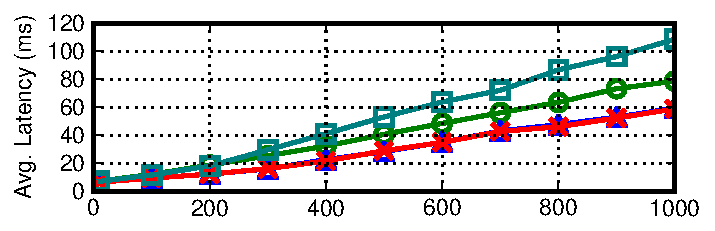
\includegraphics[width=\figfactor\columnwidth]{figs/finals/2lan-threads-lats.pdf}\vspace{-.5em}
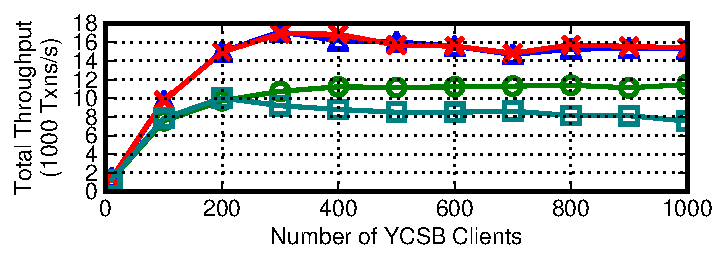
\includegraphics[width=\figfactor\columnwidth]{figs/finals/2lan-threads-thru.pdf}\vspace{-.75em}
\begin{center}\small\textbf{B.) Between \texttt{us-east} \texttt{(CA)} and \texttt{us-west-2} \texttt{(OR)}}\end{center}\vspace{-1.5em}
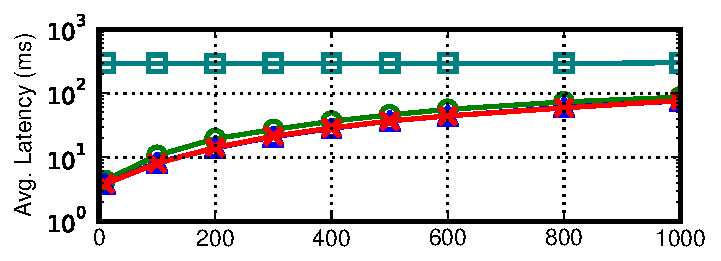
\includegraphics[width=\figfactor\columnwidth]{figs/finals/2wan-threads-lats-log.pdf}\vspace{-.5em}
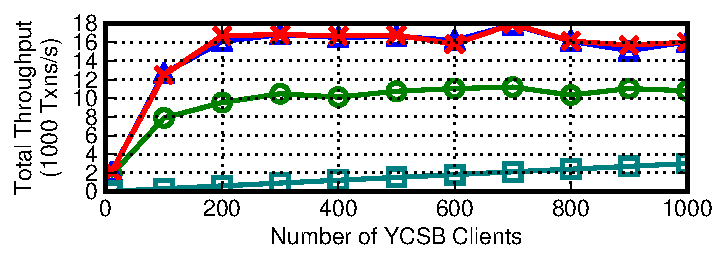
\includegraphics[width=\figfactor\columnwidth]{figs/finals/2wan-threads-thru.pdf}\vspace{-.75em}
\begin{center}\small \textbf{C.) Between}{ \texttt{us-east} \texttt{(VA)}, \texttt{us-west-1} \texttt{(CA)},\\ \texttt{us-west-2} \texttt{(OR)}, \texttt{eu-west} \texttt{(IR)}, \texttt{ap-northeast} \texttt{(SI)}}\end{center}\vspace{-1.5em}
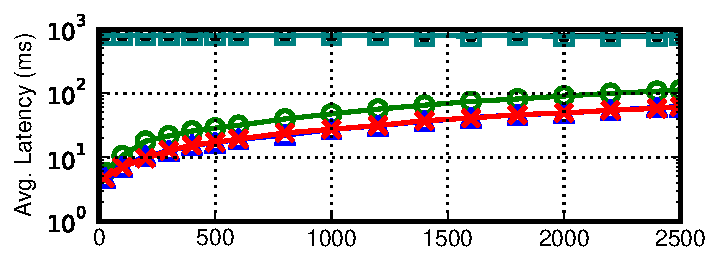
\includegraphics[width=\figfactor\columnwidth]{figs/finals/5wan-threads-lats-log.pdf}\vspace{--.5em}
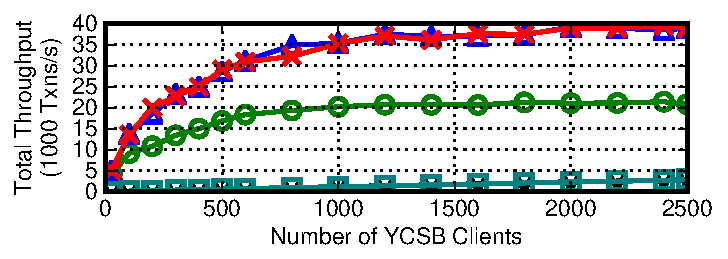
\includegraphics[width=\figfactor\columnwidth]{figs/finals/5wan-threads-thru.pdf}
\caption{YCSB performance for two clusters of five servers each
  deployed within a single datacenter and cross-datacenters.}\vspace{-1.5em}
\label{fig:wan-exp}
\end{figure}

\vspace{.5em}\noindent\textit{Geo-replication.} We first deploy the
database prototype across an increasing number of
datacenters. Figure~\ref{fig:wan-exp}A shows that, when operating two
clusters within a single datacenter, mastering each data item results
in approximately half the throughput and double the latency of
\texttt{eventual}. This is because HAT models are able to utilize
replicas in both clusters instead of always contacting the (single)
master. \texttt{RC}---essentially \texttt{eventual} with
buffering---is almost identical to \texttt{eventual}, while
\texttt{TA}---which incurs two writes for every client-side write
(i.e., new writes are sent to the WAL then subsequently moved into
LevelDB once pending stable)---achieves ~75\% of the throughput. Latency
increases linearly with the number of YCSB clients due to contention
within LevelDB.

In contrast, when the two clusters are deployed across the continental
United States (Figure~\ref{fig:wan-exp}B), the average latency of
\texttt{master} increases to $300$ms (a $278$--$4257\%$ latency
increase; average $37$ms latency per operation). For the same number
of YCSB client threads, \texttt{master} has substantially lower
throughput than the HAT configurations. Increasing the number of YCSB
clients \textit{does} increase the throughput of \texttt{master}, but
our Thrift-based server-side connection processing did not gracefully
handle more than several thousand concurrent connections. In contrast,
across two datacenters, the performance of eventual, RC, and TA are
near-identical to a single-datacenter deployment.

When five clusters (as opposed to two, as before) are deployed across
the five EC2 datacenters with lowest communication cost
(Figure~\ref{fig:wan-exp}C), the trend continues: \texttt{master}
latency increases to nearly $800$ms per transaction. As an attempt at
reducing this overhead, we implemented and benchmarked a variant of
quorum-based replication as in Dynamo~\cite{dynamo}, where clients
sent requests to all replicas, which completed as soon as a majority
of servers responded (guaranteeing regular
semantics~\cite{herlihy-art}); this strategy (not pictured) did not
substantially improve performance due to the network topology and
because worst-case server load was unaffected. With five clusters,
TA's relative throughput decreased: every YCSB \texttt{put} operation
resulted in four \texttt{put} operations on remote replicas and,
accordingly, the cost of anti-entropy increased (e.g., each server
processed four replica's anti-entropy as opposed to one before,
reducing the opportunity for batching and decreasing available
resources for incoming client requests). This in turn increased
garbage collection activity and, more importantly, IOPS when compared
to Eventual and RC, causing TA throughput to peak at around half of
Eventual. With in-memory persistence (i.e., no LevelDB or WAL),
\texttt{TA} throughput was within 20\% of \texttt{eventual}.

We have intentionally omitted performance data for two-phase
locking. \texttt{master} performed \textit{far} better than our
textbook implementation, which, in addition to requiring a WAN
round-trip per operation, also incurred substantial overheads due to
mutual exclusion via locking. We expect that, while techniques like
those recently proposed in Calvin~\cite{calvin} can reduce the
overhead of serializable transactions by avoiding locking, our
mastered implementation and the data from Section~\ref{sec:latency}
are reasonable lower bounds on latency.

\begin{figure}[t!]
\begin{center}
\hspace{2em}
\includegraphics[width=.8\columnwidth]{figs/strategylegend.pdf}\vspace{-2em}
\end{center}
\begin{center}
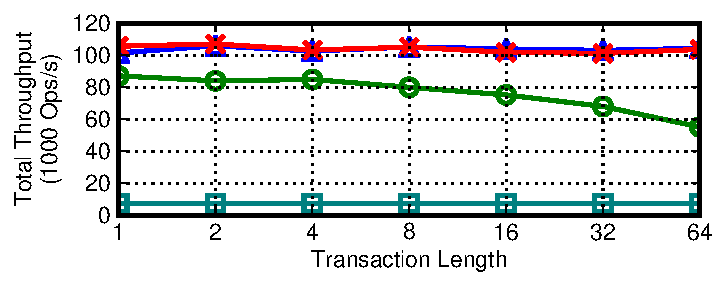
\includegraphics[width=\figfactor\columnwidth]{figs/finals/txnlen-thru.pdf}
\end{center}\vspace{-2.25em}
\caption{Transaction length versus throughput.}\vspace{-1em}
\label{fig:txlen}
\begin{center}
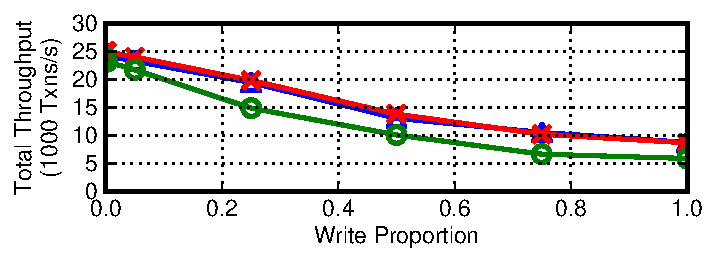
\includegraphics[width=\figfactor\columnwidth]{figs/finals/wprop-thru.pdf}
\end{center}\vspace{-2.25em}
\caption{Proportion of reads and writes versus throughput.}\vspace{-1em}
\label{fig:rprop}
\begin{center}
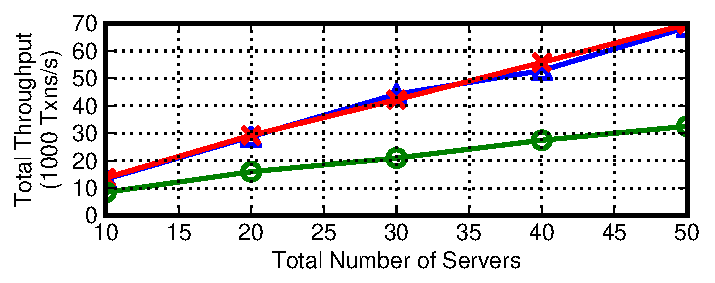
\includegraphics[width=\figfactor\columnwidth]{figs/finals/scaleout-thru.pdf}
%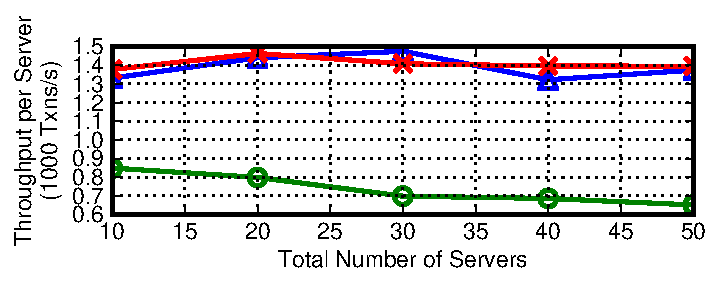
\includegraphics[width=\figfactor\columnwidth]{figs/finals/scaleout-thru-perserver.pdf}
\end{center}\vspace{-2.25em}
\caption{Scale-out of TA, Eventual, and RC.}\vspace{-1.5em}
\label{fig:scaleout}
\end{figure}

\vspace{.5em}\noindent\textit{Transaction length.} As shown in
Figure~\ref{fig:txlen} (clusters in Virginia and Oregon), throughput
of \texttt{eventual}, \texttt{RC}, and \texttt{master} operation are
unaffected by transaction length. In contrast, \texttt{TA} throughput
decreases linearly with increased transaction length: with $1$
operation per transaction, \texttt{TA} throughput is within 18\% of
\texttt{eventual} ($34$ bytes overhead), and with $128$ operations per
transaction, \texttt{TA} throughput is within $60\%$ ($1898$ bytes
overhead). This reflects our TA algorithm's metadata requirements,
which are proportional to transaction length and consume IOPS and
network bandwidth.


\vspace{.5em}\noindent\textit{Read proportion.} Our default (equal)
proportion of reads and writes is fairly pessimistic: for example,
Facebook reports $99.8\%$ reads for their workload~\cite{eiger}. As
shown in Figure~\ref{fig:rprop} (clusters in Virginia and Oregon),
with all reads, \texttt{TA} is within $4.8\%$ of \texttt{eventual};
with all writes, \texttt{TA} is within $33\%$, and the throughput of
\texttt{eventual} decreases by $288.8\%$ compared to all reads. At
$99.8\%$ reads, \texttt{TA} incurs a $7\%$ overhead ($5.8\%$ for in-memory
storage).



\vspace{.5em}\noindent\textit{Scale-out.} One of the key benefits of
our HAT algorithms is that they are shared-nothing, meaning they
should not compromise scalability. Figure~\ref{fig:scaleout} shows
that varying the number of servers across two clusters in Virginia and
Oregon (with $15$ YCSB clients per server) results in linear scale-out
for \texttt{eventual}, \texttt{RC}, and \texttt{TA}. \texttt{RC} and
\texttt{eventual} scale perfectly with an approximately $5$x
throughput increase moving from $5$ to $25$ servers per cluster. For
the same configuration, \texttt{TA} scales by $3.8$x, achieving over
$260,000$ operations per second. \texttt{TA} performance is due to
resource contention---with a memory-backed database (instead of
LevelDB), \texttt{TA} scales by $4.25$x (not shown)---and TA-related
performance heterogeneity across servers (Calvin's authors report
similar heterogeneity on EC2~\cite{calvin}). Nevertheless, this linear
scalability is not typical of traditional database system
designs~\cite{gray-isolation}.

\vspace{.5em}\noindent\textit{Summary.} Our experimental prototype
confirms our earlier analytical intuitions. HAT systems can provide
useful semantics without substantial performance penalties. In
particular, our TA algorithm can achieve throughput competitive with
eventual consistency at the expense of increased disk and network
utilization. Perhaps more importantly, all HAT algorithms circumvent
high WAN latencies inevitable with non-HAT implementations. Our results
highlight Deutsch's observation that ignoring factors such as latency
can ``cause big trouble and painful learning
experiences''~\cite{fallacies-deutsch}---in a single-site context,
paying the cost of coordination may be tenable, but, especially as
services are geo-replicated, costs increase.
